
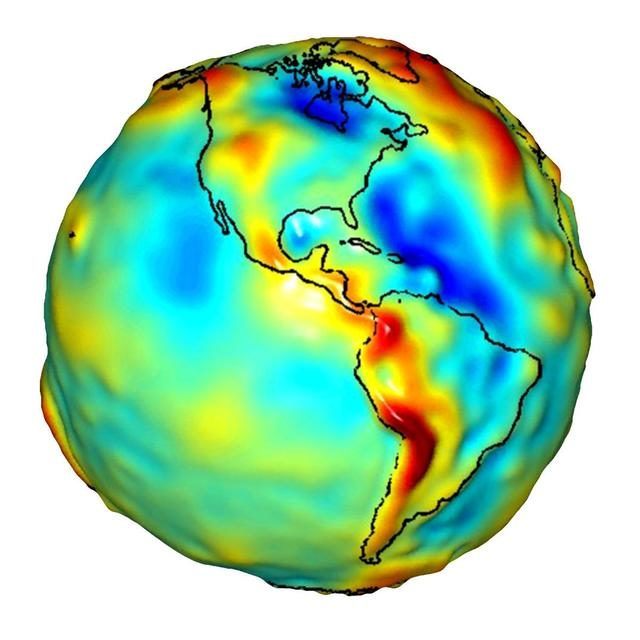
\includegraphics[height=1.5cm]{images/pictograms/gravity}

%\lstinputlisting[language=bash,basicstyle=\small]{python_codes/fieldstone_113/keywords.ascii}

\begin{center}
\inpython~Code at \url{https://github.com/cedrict/fieldstone/tree/master/python_codes/fieldstone_113}
\end{center}

\par\noindent\rule{\textwidth}{0.4pt}

%%%%%%%%%%%%%%%%%%%%%%%%%%%%%%%%%%%%%%%%%%%%%%%%%%%%%%%%%%%%%%%%%%%%%%%%%%%%%%%%%%%%%%%%%%%%%%%%%%%%

Last revision: Sept. 26th, 2024.

\par\noindent\rule{\textwidth}{0.4pt}
%%%%%%%%%%%%%%%%%%%%%%%%%%%%%%%%%%%%%%%%%%%%%%%%%%%%%%%%%%%%%%%%%%%%%%%%%%%%%%%%%%%%%%%


This \stone based on the article by Werner \& Scheeres (1997) \cite{wesc97} in which 
the gravity fields generated by a polyhedron {\it of constant density}.


Before we dive in the calculations it is worth highlighting a few excerpts from the paper. 
First, the authors present three methods to compute the gravity field of an irregular-shaped
body:
\begin{enumerate}
\item harmonic expansion. They write:
\begin{displayquote}
{\color{darkgray}
Harmonic expansions have several drawbacks. 
The first is that the harmonic expansion is always an approximation to a gravity field due to the finite
truncation of the series expansion. The truncation error grows when evaluating
the gravity field close to the model's radius of convergence. Additional terms are
necessary in the expansion to maintain a given accuracy.\\
The second major drawback is that the same form of the exterior harmonic
expansion is no longer guaranteed to converge inside the circumscribing sphere,
and indeed often diverges.\\
Another drawback is that the harmonic expansion yields no information about
whether a field point is outside or inside the body.}
\end{displayquote}

\item mass concentrations ('mascons').

\begin{displayquote}
{\color{darkgray}
A second, commonly used approach for evaluating asteroid gravitation is to fill the
body with point masses ('mascons' - mass concentrations) on an evenly spaced
grid (Geissler et al., 1995).
[...] for a given computational effort, the mascon approach is less accurate than 
a harmonic approach (in its region of convergence).}
\end{displayquote}


\item polyhedron. This is the method presented in the paper. 
\begin{displayquote}
{\color{darkgray}
we investigate a third approach, which is to model the asteroid as a
constant-density polyhedron. The polyhedron can have concavities in its surface
(e.g. craters), overhangs, interior voids (caves), and even holes all the way through
(torus). There is no special penalty for including small details, i.e. the entire body
does not have to be modeled at a uniformly high resolution.
[...] The polyhedral approach remedies several drawbacks outlined above.
The gravity field is exact for the given shape and density.
polyhedron gravitation is a valid and exact solution up to the surface of
the body. There is no region of divergence.
[...] Another way our work differs is that our ultimate formulas are expressed intrinsi-
cally using vectors and distances. Other papers are cluttered with special coordinate
systems and angles.
}
\end{displayquote}

\end{enumerate}


The authors explain what a polyhedron is in this context:
\begin{displayquote}
{\color{darkgray}
By polyhedron we mean a three-dimensional solid body whose surface consists of planar faces 
meeting along straight edges or at isolated points called vertices. Exactly two faces meet 
at each edge. Three or more edges and a like number of faces meet at each vertex. Note: 
the vertex coordinates of a polyhedron alone are insufficient to describe it. The connective 
topology must also be described -- edges connect which vertex pairs and bound which face pairs.}
\end{displayquote}

The volume integrals are transformed via the Gauss divergence theorem, into surface integrals, e.g.:
\[
U = \frac12 {\cal G} \rho_0 \iint_S \vec{n} \cdot \frac{\vec{r}}{r} \; dS
\]
Ultimately this integral will involve face integrals and edges integrals.
The paper is somewhat complex but well written. There is however no point re-typing all 
the derivations and I present in the next section the finalised equations of their Section~2.6.


%--------------------------------------------------------
\subsection*{Theory}

In what follows $e=1,2,...6$ stands for an edge while $f=1,2,3,4$ stands
for a face. 
Each polyhedron face has an outward-pointing face normal vector $\vec{n}_f$
and a face dyad ${\bm F}_f =\vec{n}_f\vec{n}_f $.
Each edge of each face has an outward-pointing edge normal
vector $\vec{n}_{e,f}$ perpendicular to both $\vec{n}_f$ and the edge.
For the edge connecting vertices 1 and 2 shared by faces A and B,
the edge dyad is ${\bm E}_{12}=\vec{n}_A \vec{n}_{12,A}+\vec{n}_B \vec{n}_{21,B}$.

Let $\vec{r}_i$ represent the vector from the variable 
field-point M at location $\vec{r}_M$ to polyhedron vertex $P_i$, 
and let $r_i = ||\vec{r}_i||$ be its length.


For the polyhedron edge connecting
vertices $i$ and $j$ of length $l_{ij}$, the dimensionless per-edge factor $L_e$ is
\[
L_e=L_{ij} = \int_e \frac{1}{r}ds = \int_{P_i}^{P_j} \frac{1}{r} ds 
= \ln \frac{r_i+r_j+l_{ij}}{r_i+r_j-l_{ij}}
\]
For a triangular face $f$ bounded by vertices $i,j,k$ the dimensionless
per-face factor $\omega_f$ is 
\[
\omega_f = 
\iint_{triangle} \frac{\Delta z}{r^3} dS 
= 2 \arctan \frac{\vec{r_i} \cdot (\vec{r}_j \times \vec{r}_k)}{r_ir_jr_k 
+r_i(\vec{r}_j\cdot\vec{r}_k) 
+r_j(\vec{r}_k\cdot\vec{r}_i) 
+r_k(\vec{r}_i\cdot\vec{r}_j) 
}
\]
The gravity vector $\vec{g}$ generated by the mass inside the tetrahedron 
at point $M$ is given by
\[
-\vec{g} = \vec\nabla U = 
- \underbrace{{\cal G} \rho_0 \sum_e L_e {\bm E}_e\cdot\vec{r}_e}_{\vec{g}_e}
+
\underbrace{{\cal G} \rho_0 \sum_f \omega_f {\bm F}_f\cdot \vec{r}_f}_{\vec{g}_f}
= -\vec{g}_e + \vec{g}_f
\]
with
\begin{eqnarray}
\vec{g}_e 
&=& {\cal G} \rho_0 \sum_e L_e {\bm E}_e \cdot \vec{r}_e \nn\\
&=& {\cal G} \rho_0 \left(
L_{12} {\bm E}_{12}\cdot\vec{r}_{12} +
L_{13} {\bm E}_{23}\cdot\vec{r}_{13} +
L_{14} {\bm E}_{34}\cdot\vec{r}_{14} \right. \nn\\
&& \left. + 
L_{23} {\bm E}_{23}\cdot\vec{r}_{23} + 
L_{24} {\bm E}_{24}\cdot\vec{r}_{24} +
L_{34} {\bm E}_{34}\cdot\vec{r}_{34} 
\right) \label{eq:tetra:ge}\\ \nn\\
\vec{g}_f
&=& {\cal G} \rho_0 \sum_f \omega_f {\bm F}_f\cdot \vec{r}_f \nn\\
&=& {\cal G} \rho_0 \left(
\omega_A {\bm F}_A\cdot \vec{r}_A +
\omega_B {\bm F}_B\cdot \vec{r}_B +
\omega_C {\bm F}_C\cdot \vec{r}_C +
\omega_D {\bm F}_D\cdot \vec{r}_D  
\right) \label{eq:tetra:gf}
\end{eqnarray}
and the gravity potential and tensor are then given by
\begin{eqnarray}
U &=& \frac12 {\cal G} \rho_0  \sum_e  L_e \; \vec{r}_e\cdot{\bm E}_e \cdot \vec{r}_e 
-\frac12 {\cal G} \rho_0 \sum_f \omega_f \; \vec{r}_f \cdot{\bm F}_f \cdot \vec{r}_f  \\
{\bm T} &=&
\vec\nabla\vec\nabla U = -\vec\nabla \vec{g} =
{\cal G} \rho_0 \sum_e 
L_e \cdot{\bm E}_e 
- {\cal G} \rho_0 \sum_f \omega_f \; {\bm F}_f 
\end{eqnarray}



Let us consider a generic tetrahedron:
\begin{center}
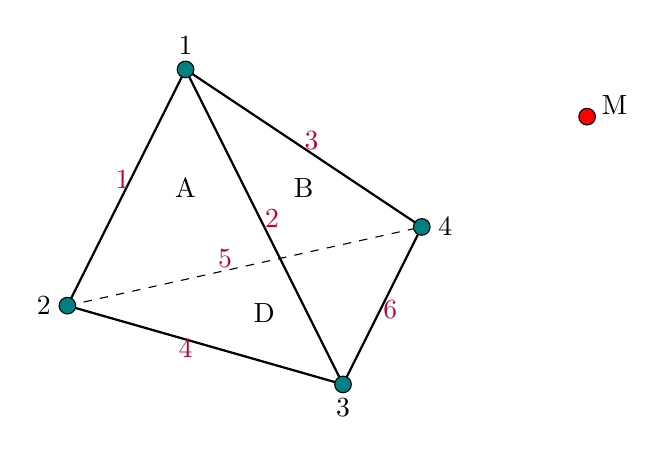
\begin{tikzpicture}
%\draw[step=0.5cm,gray,very thin] (0,0) grid (7,6); 
\draw[thick] (2.5,5) -- (1,2) -- (4.5,1) -- (5.5,3) -- cycle;
\draw[thick] (2.5,5)  -- (4.5,1) ;
\draw[dashed] (1,2) --  (5.5,3);
\node[] at (2.5,5.3) {$1$};
\node[] at (0.7,2) {$2$};
\node[] at (4.5,0.7) {$3$};
\node[] at (5.8,3) {$4$};
\draw[black,fill=teal] (2.5,5) circle (3pt);
\draw[black,fill=teal] (1,2) circle (3pt);
\draw[black,fill=teal] (4.5,1) circle (3pt);
\draw[black,fill=teal] (5.5,3) circle (3pt);
\node[] at (2.5,3.5) {A};
\node[] at (4,3.5) {B};
\node[] at (3.5,1.9) {D};
\draw[black,fill=red] (7.6,4.4) circle (3pt);
\node[] at (7.95,4.55) {M};
\node[] at (1.7,3.6) {\color{purple}1};
\node[] at (3.6,3.1) {\color{purple}2};
\node[] at (4.1,4.1) {\color{purple}3};
\node[] at (2.5,1.45) {\color{purple}4};
\node[] at (3,2.6) {\color{purple}5};
\node[] at (5.1,1.95) {\color{purple}6};
\end{tikzpicture}\\
{\captionfont Face C is hidden in the back.}
\end{center}


When looking at a face from the outside towards the tetrahedron the numbering 
of vertices is counter-clockwise.
\begin{center}
\begin{tabular}{ccccc}
\hline
face & vertices $i,j,k$ & edge \#1 & edge \#2 & edge \#3 \\
\hline\hline
A& 1,2,3  & 12({\color{purple}1}) & 23({\color{purple}4}) & 31({\color{purple}2}) \\
B& 1,3,4  & 13({\color{purple}2}) & 34({\color{purple}6}) & 41({\color{purple}3}) \\
C& 1,4,2  & 14({\color{purple}3}) & 42({\color{purple}5}) & 21({\color{purple}1}) \\
D& 2,4,3  & 24({\color{purple}5}) & 43({\color{purple}6}) & 32({\color{purple}4}) \\
\hline
edge & vertices & belongs to \\
{\color{purple}1} & 12 & A,C\\
{\color{purple}2} & 13 & A,B\\
{\color{purple}3} & 14 & B,C\\
{\color{purple}4} & 23 & A,D\\
{\color{purple}5} & 24 & C,D\\
{\color{purple}6} & 34 & B,D\\
\hline
\end{tabular}
\end{center}


\begin{center}
\begin{tikzpicture}
%\draw[step=0.5cm,gray,very thin] (0,0) grid (12,8.5); 
\draw[thick] (0.6,2.8) -- (3,5.6)--(6.7,6.9);
\draw[thick] (3,5.6)  -- (8.1,3.2) ;
\draw[thick] (5.9,0.4) -- (8.1,3.2) -- (11.1,4.2);
\node[] at (9,4.5) {face A};
\node[] at (4.5,2) {face B};
\draw[thick,->] (2.4,3.5)--(0.5,5); 
\node[] at (0.5,5.25) {$\vec{n}_B$};
\draw[] (2.2,3.65) -- (2.38,3.85) --(2.58,3.66);
\draw[thick,->] (5.5,5.7)--(5.2,8.1); 
\node[] at (5.6,8) {$\vec{n}_A$};
\draw[] (5.45,6) --(5.7,6.075) --(5.75,5.8);
\node[] at (2.7,5.7) {1};
\node[] at (8.2,2.85) {2};
\draw[black,fill=teal] (3,5.6) circle (3pt);
\draw[black,fill=teal] (8.1,3.2) circle (3pt);
\node[] at (8,5.8) {$\vec{n}_{21,B}$};
\draw[thick,->] (6.5,4)--(7.75,5.6); 
\node[] at (4,3) {$\vec{n}_{12,A}$};
\draw[thick,->] (6.5,4)--(4.1,3.2); 
\node[rotate=-25] at (5,5) {common edge};
\end{tikzpicture}\\
{\captionfont Figure made after Fig.~7 from \textcite{wesc97}.}
\end{center}



$\vec{n}_{1,A}=\vec{n}_{12,A}=(n_x,n_y)$ is such that it is perpendicular to $\vec{n}_A$ 
(it lies in the face $A$ plane), i.e. $\vec{n}_{1,A}\cdot \vec{n}_A=0$ and to edge $\#1$, i.e. 
$\vec{n}_{1,A}\cdot \vec{l}_{1}=0$. The cross product of $\vec{n}_A$ and $\vec{l}_{1}$ is 
by definition a vector perpendicular to both.
We also need to make sure it is pointing outwards. We then take the scalar product of a 
vector joining the center of the face and the middle of the 
edge under consideration. If it is negative then the normal is pointing towards the center of the 
face so it needs to be flipped.




%-------------------------------------------
\subsection*{Point mass approach}

Let us denote by $V$ the volume of the tetrahedron which 
can easily be computed:
\begin{equation}
V=\frac16 \left| (\vec{l}_{\color{purple}1} \times \vec{l}_{\color{purple}2}) \cdot \vec{l}_{\color{purple}3}\right|
\label{eq:tet:vol}
\end{equation}

\begin{center}
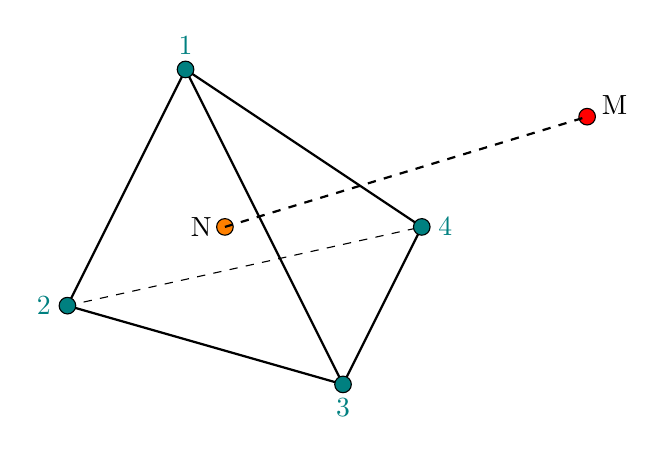
\begin{tikzpicture}
%\draw[step=0.5cm,gray,very thin] (0,0) grid (7,6); 
\draw[thick] (2.5,5) -- (1,2) -- (4.5,1) -- (5.5,3) -- cycle;
\draw[thick] (2.5,5)  -- (4.5,1) ;
\draw[dashed] (1,2) --  (5.5,3);
\node[] at (2.5,5.3) {\color{teal}$1$};
\node[] at (0.7,2) {\color{teal}$2$};
\node[] at (4.5,0.7) {\color{teal}$3$};
\node[] at (5.8,3) {\color{teal}$4$};
\draw[black,fill=teal] (2.5,5) circle (3pt);
\draw[black,fill=teal] (1,2) circle (3pt);
\draw[black,fill=teal] (4.5,1) circle (3pt);
\draw[black,fill=teal] (5.5,3) circle (3pt);

\draw[black,fill=orange] (3,3) circle (3pt);
\node[] at (2.7,3) {N};

\draw[black,fill=red] (7.6,4.4) circle (3pt);
\node[] at (7.95,4.55) {M};

\draw[thick,dashed] (3,3)--(7.6,4.4);

\end{tikzpicture}
\end{center}


The coordinates of its center of gravity $N$ (under the assumption that the 
density is constant inside it) are given by 
\begin{equation}
x_N= \frac{1}{4}(x_{\color{teal}1}+x_{\color{teal}2}+x_{\color{teal}3}+x_{\color{teal}4})
\qquad
y_N= \frac{1}{4}(y_{\color{teal}1}+y_{\color{teal}2}+y_{\color{teal}3}+y_{\color{teal}4})
\qquad
z_N= \frac{1}{4}(z_{\color{teal}1}+z_{\color{teal}2}+z_{\color{teal}3}+z_{\color{teal}4})
\label{eq:tet:centerN}
\end{equation}
If the tetrahedron is considered a point mass, then 
the gravity field and potential are given by
\begin{eqnarray}
\vec{g}_{pm} &=& {\cal G}  \frac{\rho_0 V}{|\overrightarrow{MN}|^3} \overrightarrow{MN}
\\
U_{pm} &=& {\cal G}  \frac{\rho_0 V}{|\overrightarrow{MN}|} 
\end{eqnarray}
with 
\[
\overrightarrow{MN} =
\left(
\begin{array}{c}
x_N - x_M \\
y_N - y_M \\
z_N - z_M 
\end{array}
\right)
\]

Function \verb|compute_gravity_tetrahedron_pointmass| receives coordinates of the four 
vertices {\color{teal}1}, {\color{teal}2}, {\color{teal}3}, {\color{teal}4},  its 
density and the coordinates of the measurement point.

\begin{enumerate}
\item compute coordinates $x_N,y_N,z_N$ of center of gravity with Eq.~\eqref{eq:tet:centerN}
$\rightarrow$ \verb|xN,yN,zN|

\item compute volume $V$ of tetrahedron with Eq.~\eqref{eq:tet:vol}$ \rightarrow$ \verb|Vol| 
\item compute $\vec{g}_{pm}$
\end{enumerate}

%--------------------------------
\subsection*{Full tetrahedron}

Function \verb|compute_gravity_tetrahedron| receives coordinates of the four vertices {\color{teal}1}, 
{\color{teal}2}, {\color{teal}3}, {\color{teal}4}, its density $\rho_0$ and the coordinates of the 
measurement point $M$.

I do not like the notation $\vec{e}_{12}$ for an edge vector since in fieldstone $\vec{e}$ is always 
a unit vector for the coordinate system. I then rename edge vectors $\vec{l}$.

The structure of the function goes as follows:
\begin{enumerate}
\item compute $\vec{l}_{\color{purple}1}$, $\vec{l}_{\color{purple}2}$,etc ... and their norms 
$\rightarrow$ \verb|vec_l1|, \verb|vec_l2|, \verb|vec_l3|, \verb|vec_l4|, \verb|vec_l5|, \verb|vec_l6|

\[
\vec{l}_{\color{purple}1} = \vec{l}_{\color{teal}12} = \left(
\begin{array}{c}
x_{\color{teal}2}-x_{\color{teal}1} \\
y_{\color{teal}2}-y_{\color{teal}1} \\
z_{\color{teal}2}-z_{\color{teal}1}
\end{array}
\right)
\qquad
\vec{l}_{\color{purple}2} = \vec{l}_{\color{teal}13} = \left(
\begin{array}{c}
x_{\color{teal}3}-x_{\color{teal}1} \\
y_{\color{teal}3}-y_{\color{teal}1} \\
z_{\color{teal}3}-z_{\color{teal}1}
\end{array}
\right)
\qquad
\textrm{etc...}
\]


\item compute $\vec{r}_{\color{teal} 1,2,3,4}$. $\rightarrow$ \verb|vec_r1|, \verb|vec_r2|, \verb|vec_r3|, \verb|vec_r4|
\[
\vec{r}_{\color{teal}1} = \vec{M1} = \left(
\begin{array}{c}
x_{\color{teal}1}-x_m \\
y_{\color{teal}1}-y_m \\
z_{\color{teal}1}-z_m
\end{array}
\right)
\]



\item compute $\vec{n}_{A,B,C,D}$. 
$\rightarrow$ \verb|vec_nA| , \verb|vec_nB|, \verb|vec_nC|, \verb|vec_nD|

\begin{eqnarray}
\vec{n}_A 
&=& \vec{l}_{\color{teal}12}\times\vec{l}_{\color{teal}13}/|\vec{l}_{\color{teal}12}\times\vec{l}_{\color{teal}13}|
= \vec{l}_{\color{purple}1}\times\vec{l}_{\color{purple}2}/| \vec{l}_{\color{purple}1}\times\vec{l}_{\color{purple}2}| \\
\vec{n}_B 
&=& \vec{l}_{\color{teal}13}\times\vec{l}_{\color{teal}14}/|\vec{l}_{\color{teal}13}\times\vec{l}_{\color{teal}14}|
= \vec{l}_{\color{purple}2}\times\vec{l}_{\color{purple}3}/|\vec{l}_{\color{purple}2}\times\vec{l}_{\color{purple}3}|  \\
\vec{n}_C 
&=& \vec{l}_{\color{teal}14}\times\vec{l}_{\color{teal}12}/|\vec{l}_{\color{teal}14}\times\vec{l}_{\color{teal}12}|   
= \vec{l}_{\color{purple}3}\times\vec{l}_{\color{purple}1}/|\vec{l}_{\color{purple}3}\times\vec{l}_{\color{purple}1}|   \\
\vec{n}_D 
&=& \vec{l}_{\color{teal}24}\times\vec{l}_{\color{teal}23}/|\vec{l}_{\color{teal}24}\times\vec{l}_{\color{teal}23}|   
= \vec{l}_{\color{purple}5}\times\vec{l}_{\color{purple}4}/|\vec{l}_{\color{purple}5}\times\vec{l}_{\color{purple}4}|
\end{eqnarray}


\item compute ${\bm F}_{A,B,C,D}$. 
$\rightarrow$ \verb|mat_FA| , \verb|mat_FB|, \verb|mat_FC|, 
\verb|mat_FD|

\begin{eqnarray}
{\bm F}_A &=& \vec{n}_A\vec{n}_A \\
{\bm F}_B &=& \vec{n}_B\vec{n}_B \\
{\bm F}_C &=& \vec{n}_C\vec{n}_C \\
{\bm F}_D &=& \vec{n}_D\vec{n}_D 
\end{eqnarray}

\item compute $\omega_{A,B,C,D}$. $\rightarrow$ \verb|wA| , \verb|wB|, \verb|wC|, \verb|wD|

\begin{eqnarray}
\omega_A &=& 
2 \arctan \frac{\vec{r_{\color{teal}1}} \cdot (\vec{r}_{\color{teal}2} \times \vec{r}_{\color{teal}3})}{r_{\color{teal}1}r_{\color{teal}2}r_{\color{teal}3} 
+r_{\color{teal}1}(\vec{r}_{\color{teal}2}\cdot\vec{r}_{\color{teal}3}) 
+r_{\color{teal}2}(\vec{r}_{\color{teal}3}\cdot\vec{r}_{\color{teal}1}) 
+r_{\color{teal}3}(\vec{r}_{\color{teal}1}\cdot\vec{r}_{\color{teal}2})  } \nn\\
\omega_B &=& 
2 \arctan \frac{\vec{r_{\color{teal}1}} \cdot (\vec{r}_{\color{teal}3} \times \vec{r}_{\color{teal}4})}{r_{\color{teal}1}r_{\color{teal}3}r_{\color{teal}4} 
+r_{\color{teal}1}(\vec{r}_{\color{teal}3}\cdot\vec{r}_{\color{teal}4}) 
+r_{\color{teal}3}(\vec{r}_{\color{teal}4}\cdot\vec{r}_{\color{teal}1}) 
+r_{\color{teal}4}(\vec{r}_{\color{teal}1}\cdot\vec{r}_{\color{teal}3})  } \nn\\
\omega_C &=&
2 \arctan \frac{\vec{r_{\color{teal}1}} \cdot (\vec{r}_{\color{teal}4} \times \vec{r}_{\color{teal}2})}{r_{\color{teal}1}r_{\color{teal}4}r_{\color{teal}2}
+r_{\color{teal}1}(\vec{r}_{\color{teal}4}\cdot\vec{r}_{\color{teal}2}) 
+r_{\color{teal}4}(\vec{r}_{\color{teal}2}\cdot\vec{r}_{\color{teal}1}) 
+r_{\color{teal}2}(\vec{r}_{\color{teal}1}\cdot\vec{r}_{\color{teal}4}) 
} \nn\\
\omega_D &=&
2 \arctan \frac{\vec{r_{\color{teal}2}} \cdot (\vec{r}_{\color{teal}4} \times \vec{r}_{\color{teal}3})}{r_{\color{teal}2}r_{\color{teal}4}r_{\color{teal}3} 
+r_{\color{teal}2}(\vec{r}_{\color{teal}4}\cdot\vec{r}_{\color{teal}3}) 
+r_{\color{teal}4}(\vec{r}_{\color{teal}3}\cdot\vec{r}_{\color{teal}2}) 
+r_{\color{teal}3}(\vec{r}_{\color{teal}2}\cdot\vec{r}_{\color{teal}4}) 
}
\end{eqnarray}


\item compute $\vec{r}_{A}$, $\vec{r}_{B}$, $\vec{r}_{C}$, $\vec{r}_{D}$.
As explained in the caption of their Figure~3, ``vector $\vec{r}_f$
extends from the field point $M$ to any point in the face plane''.
$\rightarrow$ \verb|vec_rA|, \verb|vec_rB|, \verb|vec_rC|, \verb|vec_rD|

\item compute $\vec{g}_f$ by means of % Eq.~\eqref{eq:tetra:gf}

\[
\vec{g}_f
= {\cal G} \rho_0 \sum_f \omega_f {\bm F}_f\cdot \vec{r}_f 
= {\cal G} \rho_0 \left(
\omega_A {\bm F}_A\cdot \vec{r}_A +
\omega_B {\bm F}_B\cdot \vec{r}_B +
\omega_C {\bm F}_C\cdot \vec{r}_C +
\omega_D {\bm F}_D\cdot \vec{r}_D 
\right)
\]




\item compute $\vec{n}_{e,f}$ for each edge of each face (12 vectors!)
$\rightarrow$ \verb|vec_nA12|, \verb|vec_nA23|, \verb|vec_nA13|, \verb|vec_nB13|, etc ...


\item compute ${\bm E}_{\color{purple} 1,2,3,4,5,6}$. 
$\rightarrow$ \verb|mat_E12, mat_E13, mat_E14, mat_E23, mat_E24, mat_E34| 

\begin{eqnarray}
{\bm E}_{\color{purple}1} ={\bm E}_{\color{teal}12}
&=&\vec{n}_A \vec{n}_{{\color{teal}12},A} +\vec{n}_C \vec{n}_{{\color{teal}21},C}\\
{\bm E}_{\color{purple}2} ={\bm E}_{\color{teal}13}
&=& \vec{n}_A \vec{n}_{{\color{teal}13},A} +\vec{n}_B \vec{n}_{{\color{teal}13},B} \\
{\bm E}_{\color{purple}3} ={\bm E}_{\color{teal}14}
&=& \vec{n}_B \vec{n}_{{\color{teal}14},B}+\vec{n}_C \vec{n}_{{\color{teal}14},C} \\
{\bm E}_{\color{purple}4} ={\bm E}_{\color{teal}23}
&=& \vec{n}_A \vec{n}_{{\color{teal}23},A}+\vec{n}_D \vec{n}_{{\color{teal}23},D} \\
{\bm E}_{\color{purple}5} ={\bm E}_{\color{teal}24}
&=& \vec{n}_C \vec{n}_{{\color{teal}24},C} +\vec{n}_D \vec{n}_{{\color{teal}24},D} \\  
{\bm E}_{\color{purple}6} ={\bm E}_{\color{teal}34}
&=& \vec{n}_B \vec{n}_{{\color{teal}34},B} +\vec{n}_D \vec{n}_{{\color{teal}34},D} 
\end{eqnarray}



\item compute $L_{\color{purple}1,2,3,4,5,6}$ $\rightarrow$ \verb|L12|, \verb|L13|, \verb|L14|, ...
\begin{eqnarray}
L_{\color{purple}1} = L_{\color{teal}12} 
&=& \ln \frac{r_{\color{teal}1}+r_{\color{teal}2}+l_{\color{purple}1}}{r_{\color{teal}1}+r_{\color{teal}2}-l_{\color{purple}1}} \nn\\
L_{\color{purple}2} = L_{\color{teal}13} 
&=& \ln \frac{r_{\color{teal}1}+r_{\color{teal}3}+l_{\color{purple}2}}{r_{\color{teal}1}+r_{\color{teal}3}-l_{\color{purple}2}} \nn\\
L_{\color{purple}3} = L_{\color{teal}14} 
&=& \ln \frac{r_{\color{teal}1}+r_{\color{teal}4}+l_{\color{purple}3}}{r_{\color{teal}1}+r_{\color{teal}4}-l_{\color{purple}3}} \nn\\
L_{\color{purple}4} = L_{\color{teal}23} 
&=& \ln \frac{r_{\color{teal}2}+r_{\color{teal}3}+l_{\color{purple}4}}{r_{\color{teal}2}+r_{\color{teal}3}-l_{\color{purple}4}} \nn\\
L_{\color{purple}5} = L_{\color{teal}24} 
&=& \ln \frac{r_{\color{teal}2}+r_{\color{teal}4}+l_{\color{purple}5}}{r_{\color{teal}2}+r_{\color{teal}4}-l_{\color{purple}5}} \nn\\
L_{\color{purple}6} = L_{\color{teal}34} 
&=& \ln \frac{r_{\color{teal}3}+r_{\color{teal}4}+l_{\color{purple}6}}{r_{\color{teal}3}+r_{\color{teal}4}-l_{\color{purple}6}} \nn
\end{eqnarray}


\item compute $\vec{r}_{\color{teal}12,13,14,23,24,34}$. As specified in Section~2.1.8 of their 
paper ``$\vec{r}_e$ is a vector from the field point to any point on edge $e$ or its infinite extension''
$\rightarrow$ \verb|vec_r12|, \verb|vec_r13|, \verb|vec_r13|, etc ...  


\item compute $\vec{g}_e$ by means of Eq.~\eqref{eq:tetra:ge}

\[
\vec{g}_e 
={\cal G} \rho_0 \sum_e L_e {\bm E}_e \cdot \vec{r}_e 
={\cal G} \rho_0 \left( 
L_{\color{teal}12} {\bm E}_{\color{teal}12}\cdot\vec{r}_{\color{teal}12} +
L_{\color{teal}13} {\bm E}_{\color{teal}23}\cdot\vec{r}_{\color{teal}13} +
L_{\color{teal}14} {\bm E}_{\color{teal}34}\cdot\vec{r}_{\color{teal}14} +
L_{\color{teal}23} {\bm E}_{\color{teal}23}\cdot\vec{r}_{\color{teal}23} 
L_{\color{teal}24} {\bm E}_{\color{teal}24}\cdot\vec{r}_{\color{teal}24} 
L_{\color{teal}34} {\bm E}_{\color{teal}34}\cdot\vec{r}_{\color{teal}34} 
\right)
\]


\item compute $\vec{g}=-\vec{g}_e+\vec{g}_f$

\end{enumerate}

Except for the 4 measurements provided in \textcite{mequ86} I could not easily find 
actual values to benchmark the code against, so the following three examples aim at 
remedying this problem. 
In all what follows we set $\rho_0=1$ and ${\cal G}=1$ for simplicity.

%..............................................
\subsection*{Test 1: the Wikipedia tetrahedron}

We consider the following regular tetrahedron (i.e. all faces are equilateral triangles) centered at the 
origin\footnote{\url{https://en.wikipedia.org/wiki/Tetrahedron}}. Its edges are $l=\sqrt{8/3}$ long.
We have
\begin{eqnarray}
(x_1,y_1,z_1) &=& (0,0,1) \nn\\
(x_2,y_2,z_2) &=& (\sqrt{8/9},0,-1/3) \nn\\
(x_3,y_3,z_3) &=& (-\sqrt{2/9},\sqrt{2/3},-1/3) \nn\\
(x_4,y_4,z_4) &=& (-\sqrt{2/9},-\sqrt{2/3},-1/3) \nn
\end{eqnarray}
Point 1 is at the top and points 2,3,4 are in the $z=-1/3$ plane.

\begin{center}
\includegraphics[width=5cm]{python_codes/fieldstone_113/images/tet1}
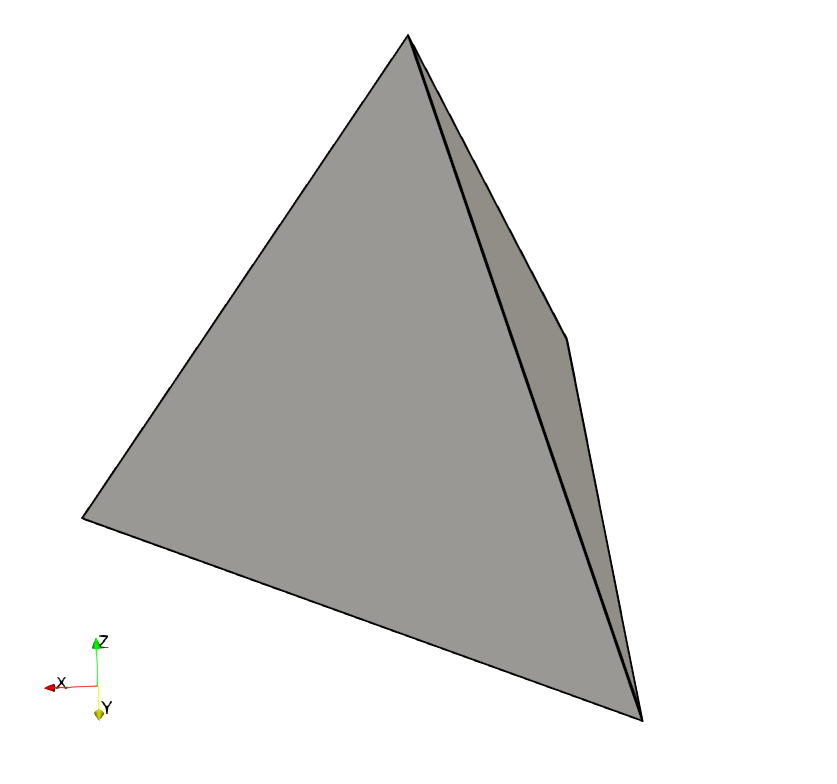
\includegraphics[width=4cm]{python_codes/fieldstone_113/results/test1/tet}
\end{center}

The volume of a regular tetrahedron of edge $l$ is given by:
\[
V=\frac{l^3}{6\sqrt{2}} = \frac{8}{9\sqrt{3}} \simeq 0.5132
\]
and this is what we indeed recover.

\begin{lstlisting}
pt_meas = np.array([0,0,10],dtype=np.float64)
pt_one=np.array([0,0,1],dtype=np.float64)
pt_two=np.array([-np.sqrt(2/9),-np.sqrt(2/3),-1/3],dtype=np.float64)
pt_three=np.array([np.sqrt(8/9),0,-1/3],dtype=np.float64)
pt_four=np.array([-np.sqrt(2/9),np.sqrt(2/3),-1/3],dtype=np.float64)
\end{lstlisting}

\begin{center}
\includegraphics[width=8cm]{python_codes/fieldstone_113/results/test1/g_vector.pdf}
\includegraphics[width=8cm]{python_codes/fieldstone_113/results/test1/g_vector_diff.pdf}\\
\includegraphics[width=8cm]{python_codes/fieldstone_113/results/test1/g_pot.pdf}
\includegraphics[width=8cm]{python_codes/fieldstone_113/results/test1/g_pot_diff.pdf}
\end{center}

%..............................................
\subsection*{Test 2: the 111-tetrahedron}

It is defined in \textcite{mequ86} (1986) (with a correction by \textcite{camq86} (1986)).

\begin{center}
\includegraphics[width=8cm]{python_codes/fieldstone_113/images/mequ86a}
\end{center}

\begin{lstlisting}
alpha=1.
pt_meas = np.array([2,0.5,0.5],dtype=np.float64)
pt_one=np.array([alpha,alpha,alpha],dtype=np.float64)
pt_two=np.array([alpha,0,0],dtype=np.float64)
pt_three=np.array([0,alpha,0],dtype=np.float64)
pt_four=np.array([0,0,alpha],dtype=np.float64)
\end{lstlisting}


In this case I choose pt1 is node C, pt2 is H, pt3 is F pt 4 is A.
If the cube is a unit cube then the edge length is $\sqrt{2}$ and the volume
\[
V=\frac{l^3}{6\sqrt{2}} = \frac13
\]

\begin{center}
\includegraphics[width=5cm]{python_codes/fieldstone_113/images/tet2}
\end{center}

\textcite{mequ86} state: ``To ensure that the above analysis can be treated
with confidence we have performed numerical calculations of the field components Fx, Fy, and 
Fz using the expressions developed in this paper and
have compared them with those obtained by direct numerical integration'':
\begin{center}
\includegraphics[width=7cm]{python_codes/fieldstone_113/images/mequ86b}\\
{\captionfont Taken from \textcite{mequ86}.}
\end{center}

\begin{center}
\begin{tabular}{lllcc}
\hline
$x$ & $y$ & $z$ & $g_x$ (tet) & $g_x$ (point mass) \\
\hline
\hline
1.25 & 0.5 & 0.5 &  0.566679144260546  & 0.5925925925925926 \\
1.5  & 0.5 & 0.5 &  0.326526930616740  & 0.3333333333333333 \\
1.75 & 0.5 & 0.5 &  0.211222015971550  & 0.2133333333333333 \\
2.0  & 0.5 & 0.5 &  0.147377525744174  & 0.1481481481481481 \\
\hline
\end{tabular}\\
Results obtained with this \stone.
\end{center}

Gravity fields are measured on a line starting at $(1,0.456,0.567)$ and ending at $(5,0.456,0.567)$
\begin{center}
\includegraphics[width=8cm]{python_codes/fieldstone_113/results/test2/g_vector.pdf}
\includegraphics[width=8cm]{python_codes/fieldstone_113/results/test2/g_vector_diff.pdf}\\
\includegraphics[width=8cm]{python_codes/fieldstone_113/results/test2/g_pot.pdf}
\includegraphics[width=8cm]{python_codes/fieldstone_113/results/test2/g_pot_diff.pdf}
\end{center}


%..........................................
\subsection*{Test 3: the origin tetrahedron}

This is not a regular tetrahedron since $l_{1} \neq l_4 $.

\begin{center}
\includegraphics[width=5cm]{python_codes/fieldstone_113/images/tet3}
\end{center}


\begin{eqnarray}
(x_1,y_1,z_1) &=& (0,0,0) \nn\\
(x_2,y_2,z_2) &=& (1,0,0) \nn\\ 
(x_3,y_3,z_3) &=& (0,1,0) \nn\\
(x_4,y_4,z_4) &=& (0,0,1) \nn
\end{eqnarray}

The gravity fields are measured on a line starting at $(1,1,1)$ and ending at $(3,3,3)$:

\begin{center}
\includegraphics[width=7cm]{python_codes/fieldstone_113/results/test3/g_vector.pdf}
\includegraphics[width=7cm]{python_codes/fieldstone_113/results/test3/g_vector_diff.pdf}\\
\includegraphics[width=7cm]{python_codes/fieldstone_113/results/test3/g_pot.pdf}
\includegraphics[width=7cm]{python_codes/fieldstone_113/results/test3/g_pot_diff.pdf}
\end{center}


%.................................................
\subsection*{Test 4: cube containing 5 tetrahedra}

{\color{red} to do!}


%..............................................
\subsection*{Test 5: sphere made of tetrahedra}



{\color{red} to do!}





